\section{Optimisations}
\subsection{WebMGA 3.0 Implementation}
\subsubsection{Distance Based Levels of Detail}
\label{optim_lod}
WebMGA 3.0 now utilises distance based variable LOD. This is implemented using three.js' built in LOD class \cite{lod_three} which acts as if it were a regular three geometry, except three.js automatically switches meshes at set camera distances. Meshes are generated at each LOD level up to the Level of Detail setting selected by the user and added to the LOD object with some distance as shown by this code,
\begin{lstlisting}
  lod_object.addLevel(mesh, distance)
\end{lstlisting}.

Lower detail meshes are used at further distances, with the distances selected by manual tuning such that the geometry change is difficult to observe. Examples of this works are shown in \cref{fig:lod_distances,fig:lod_spin}.
\begin{figure}
  \begin{center}
    \begin{subfigure}{0.3\textwidth}
      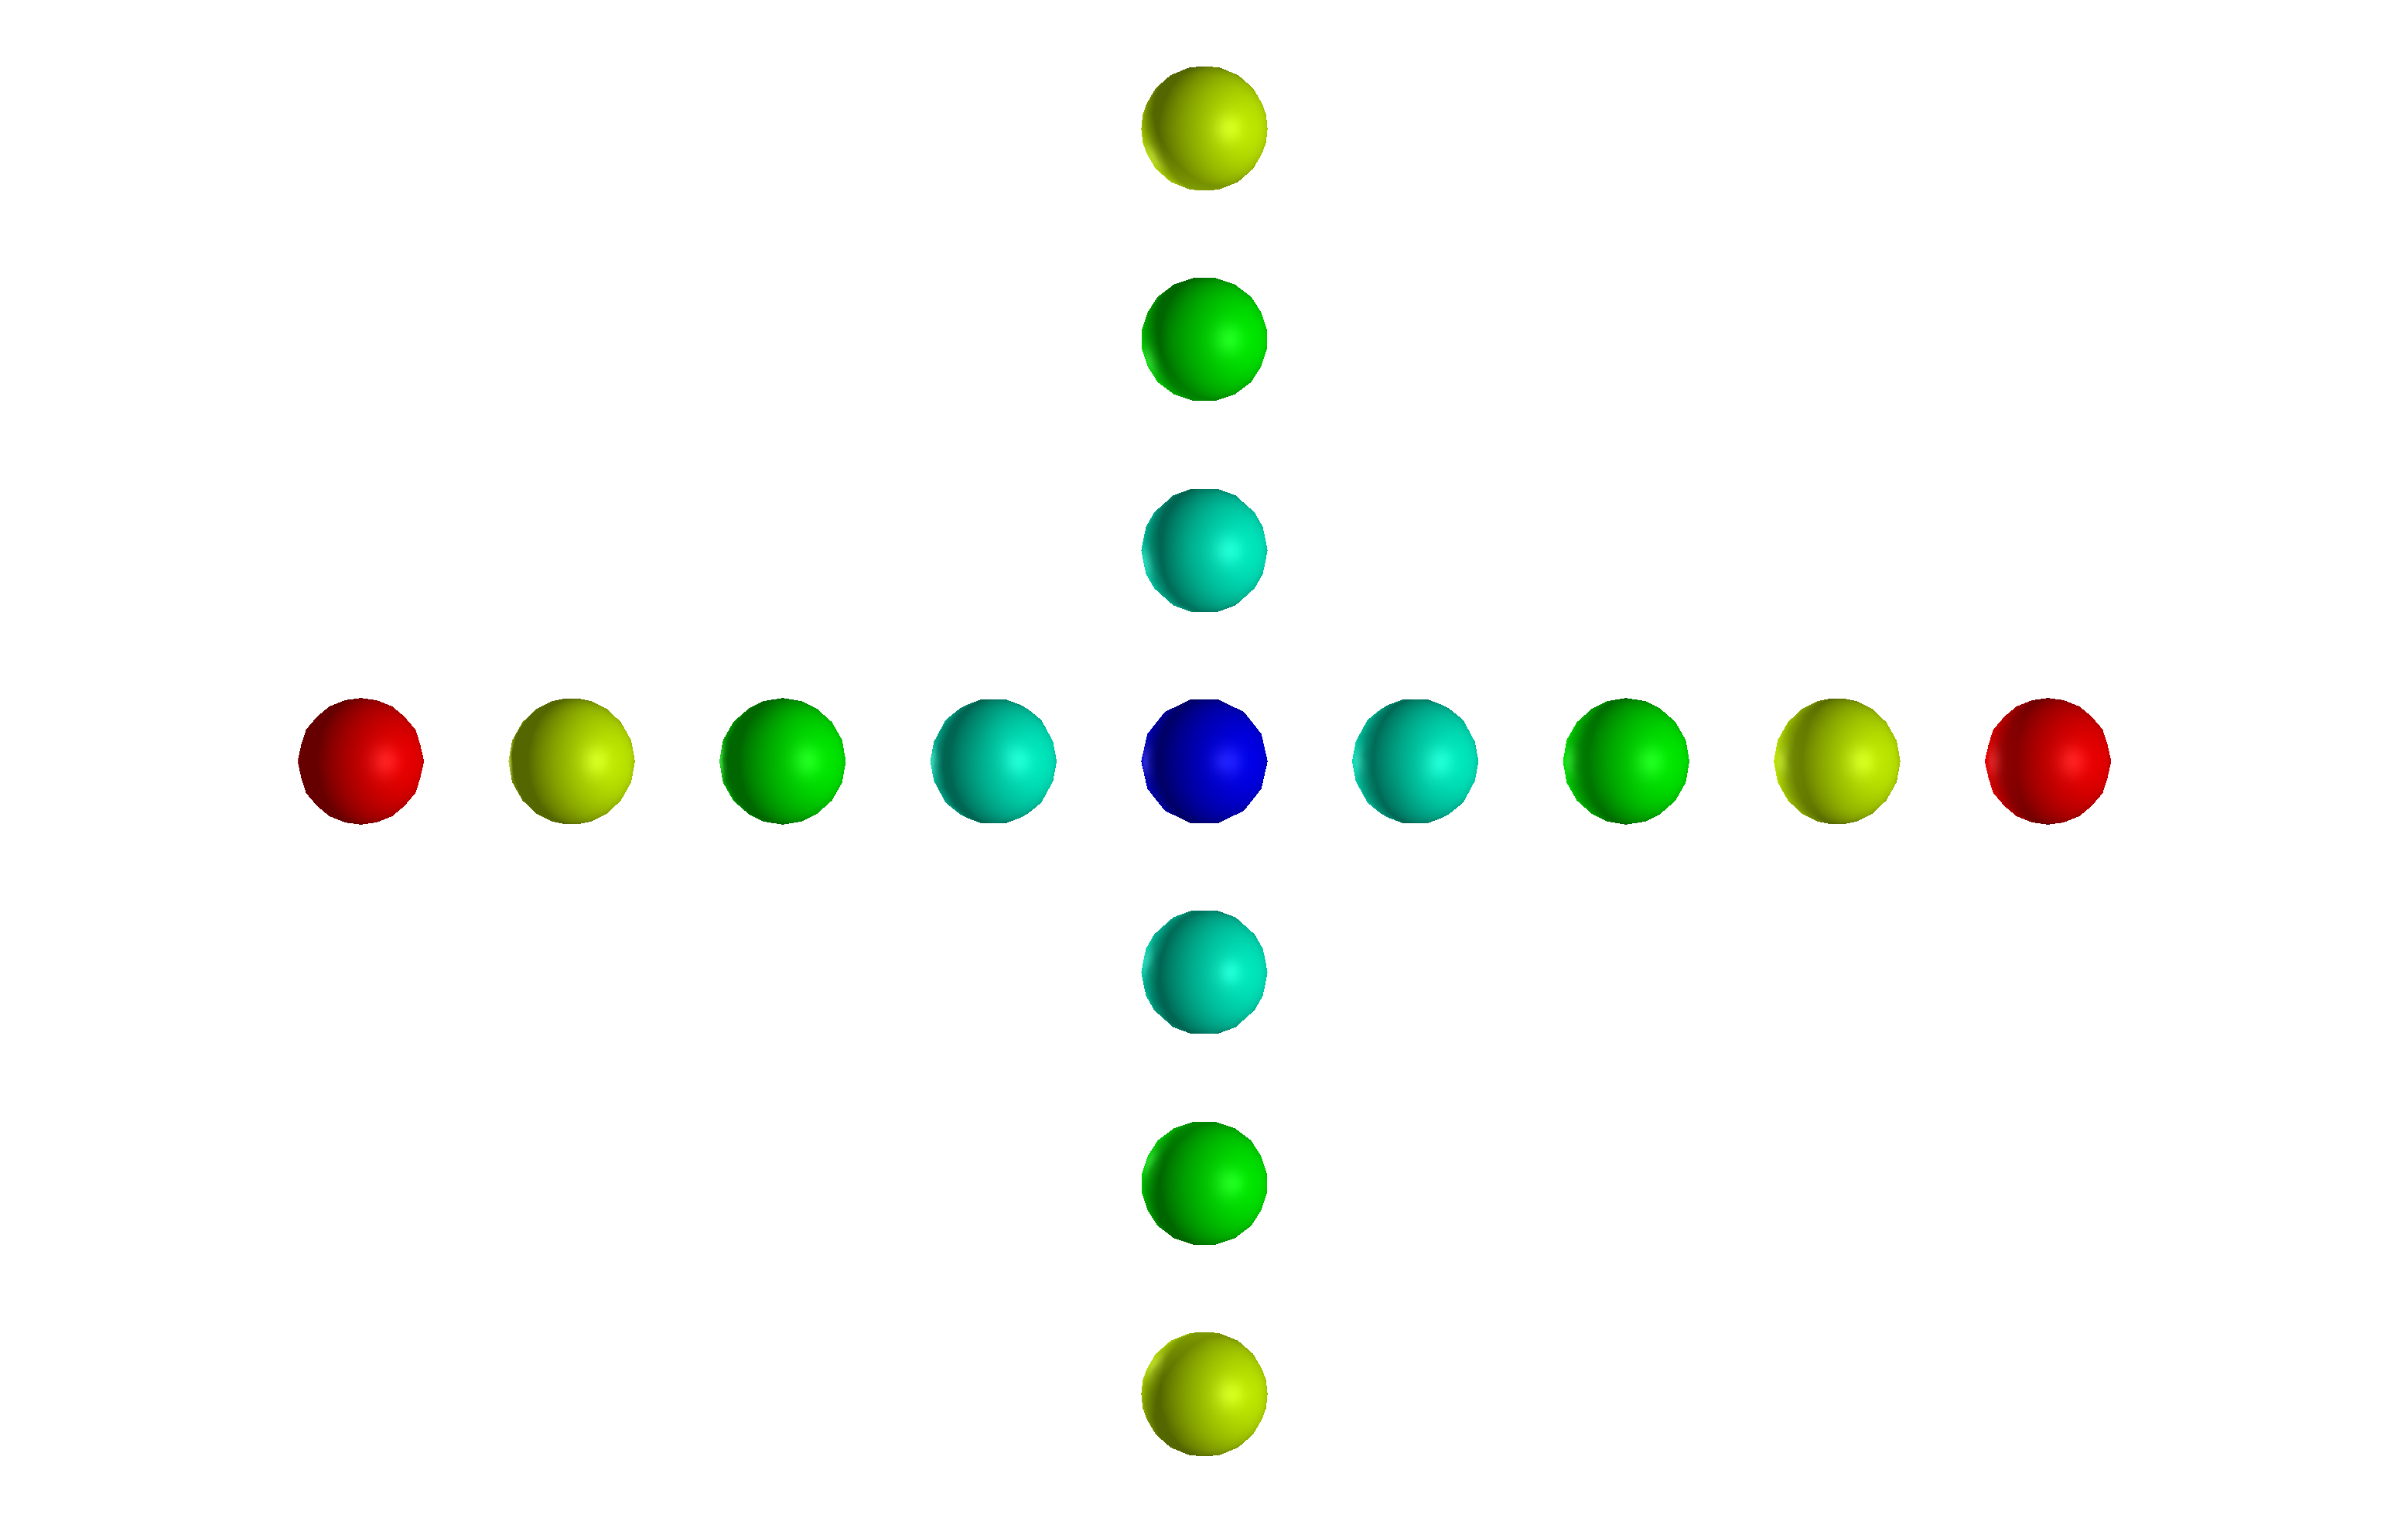
\includegraphics[width=\textwidth]{assets/images/lod/1}
      \caption{Low detail.}
      \label{fig:lod_1}
    \end{subfigure}
    \begin{subfigure}{0.3\textwidth}
      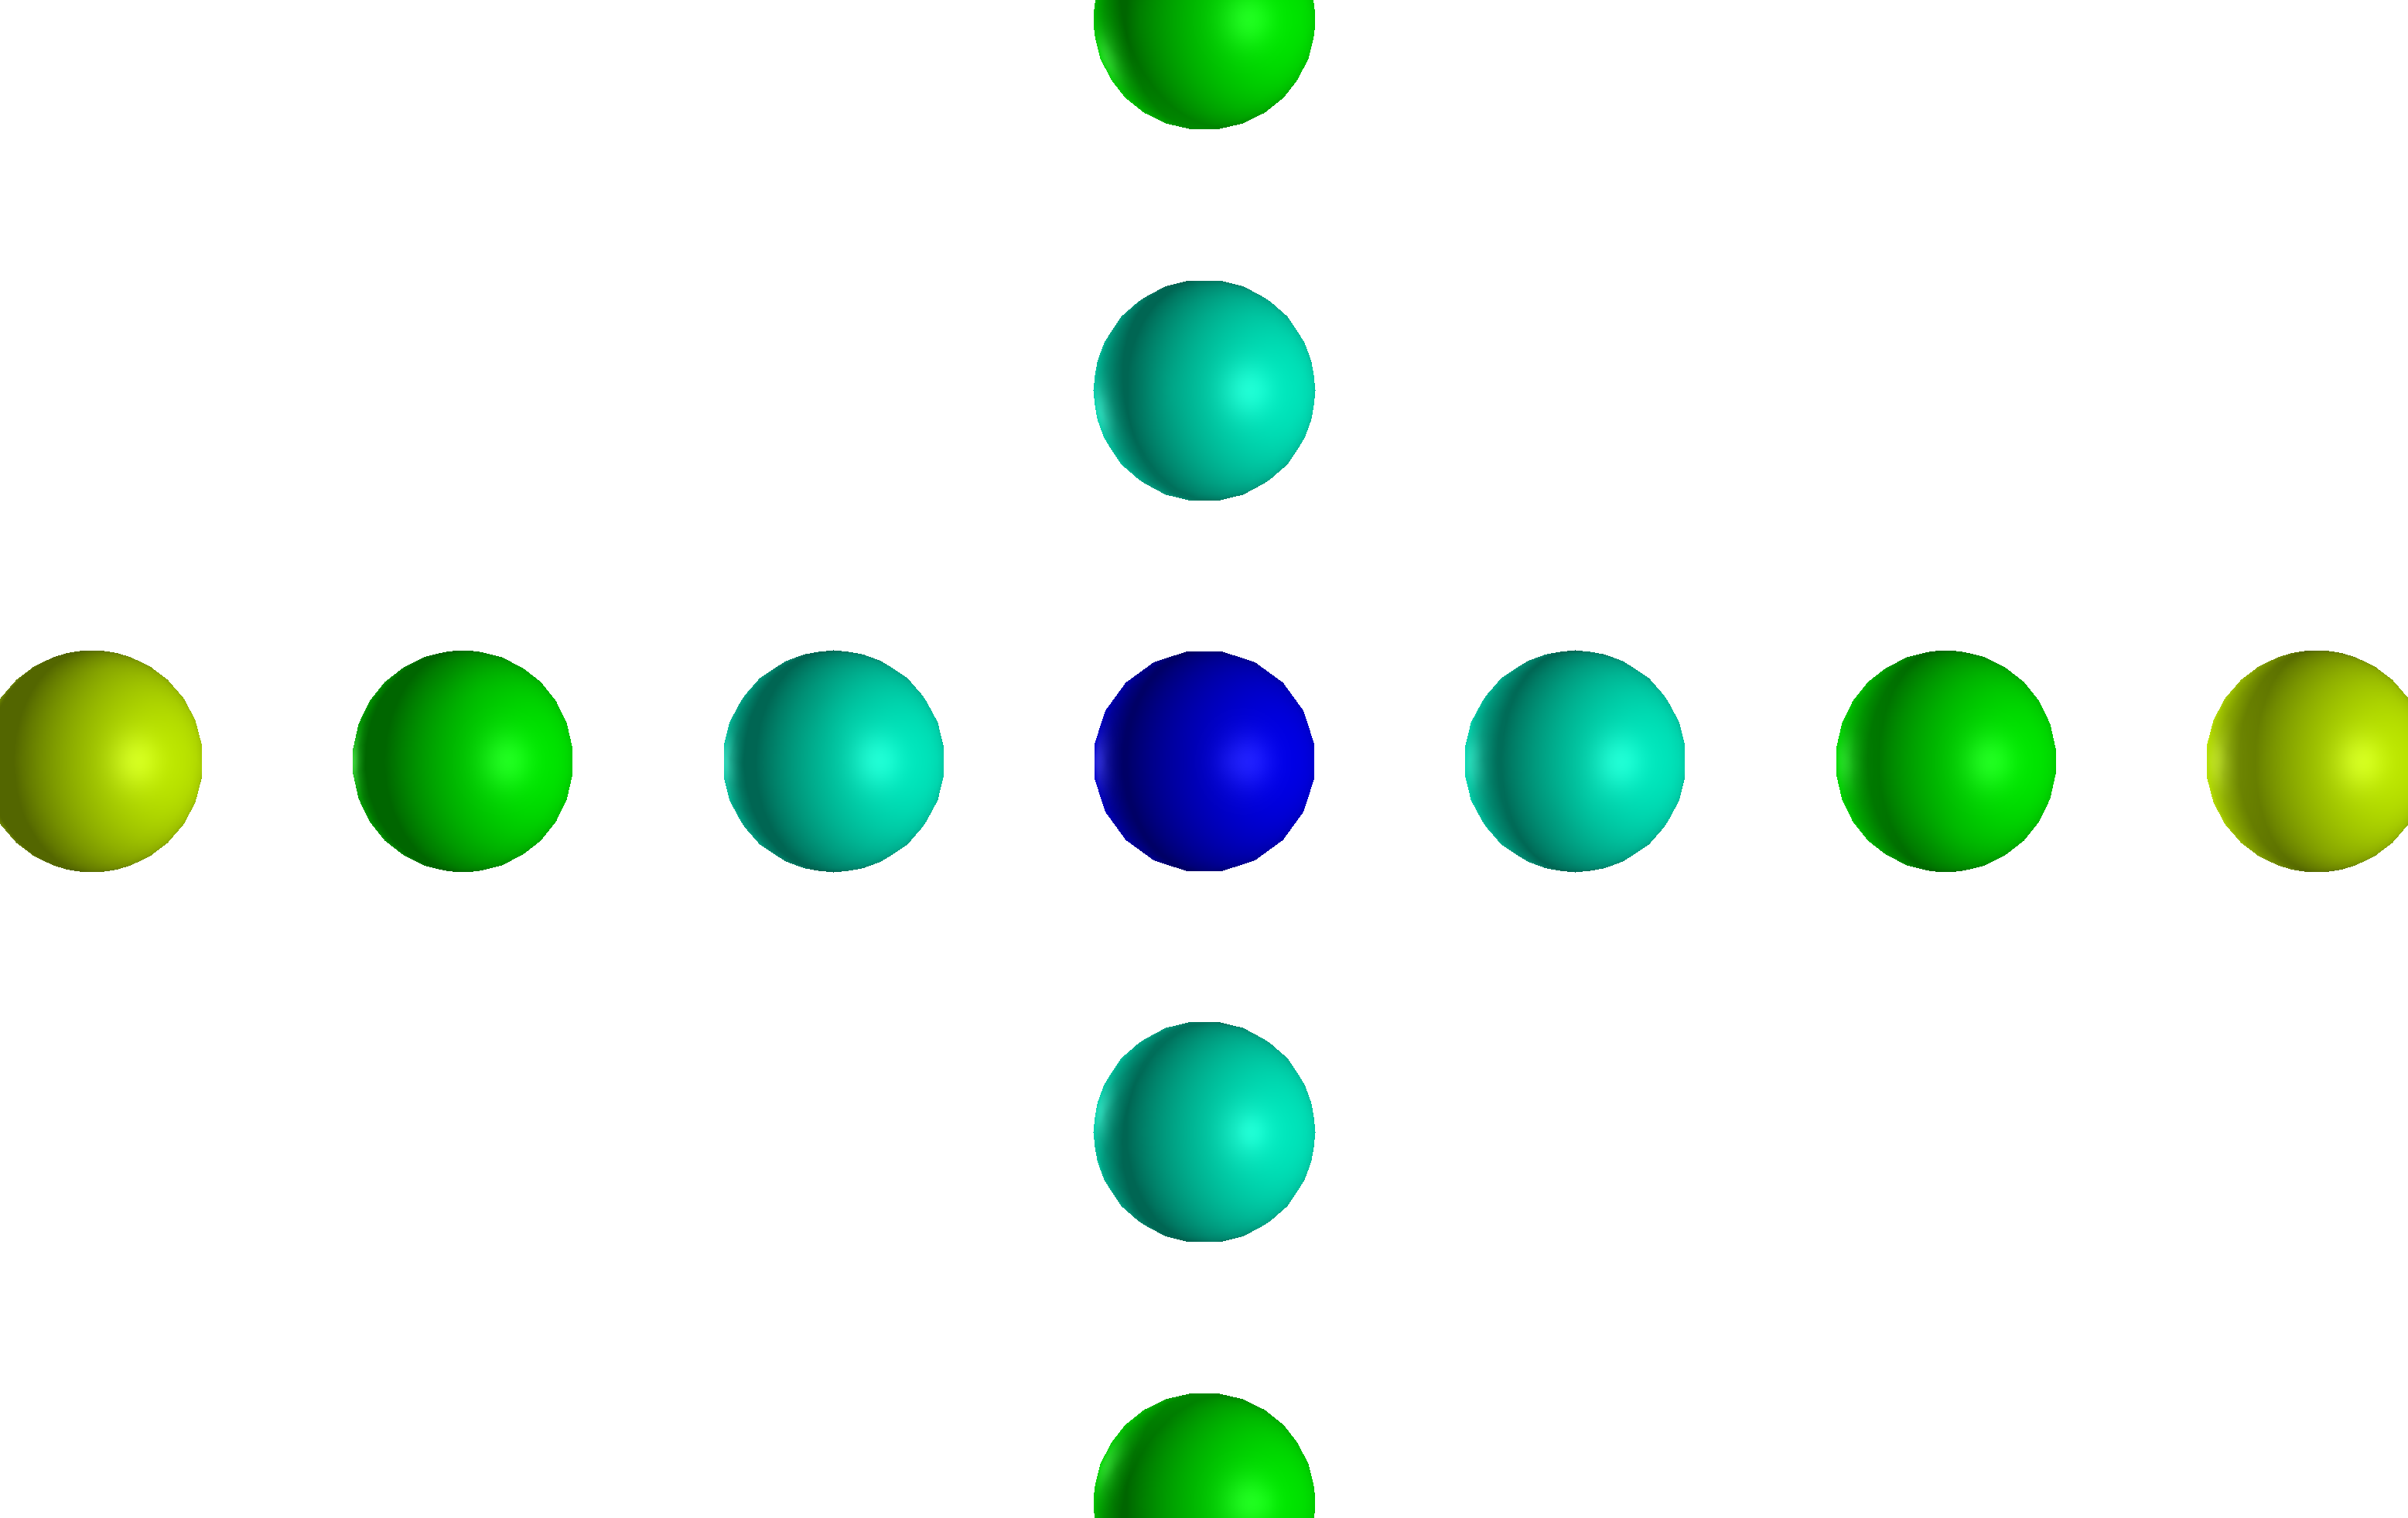
\includegraphics[width=\textwidth]{assets/images/lod/2}
      \caption{Medium detail.}
      \label{fig:lod_2}
    \end{subfigure}
    \begin{subfigure}{0.3\textwidth}
      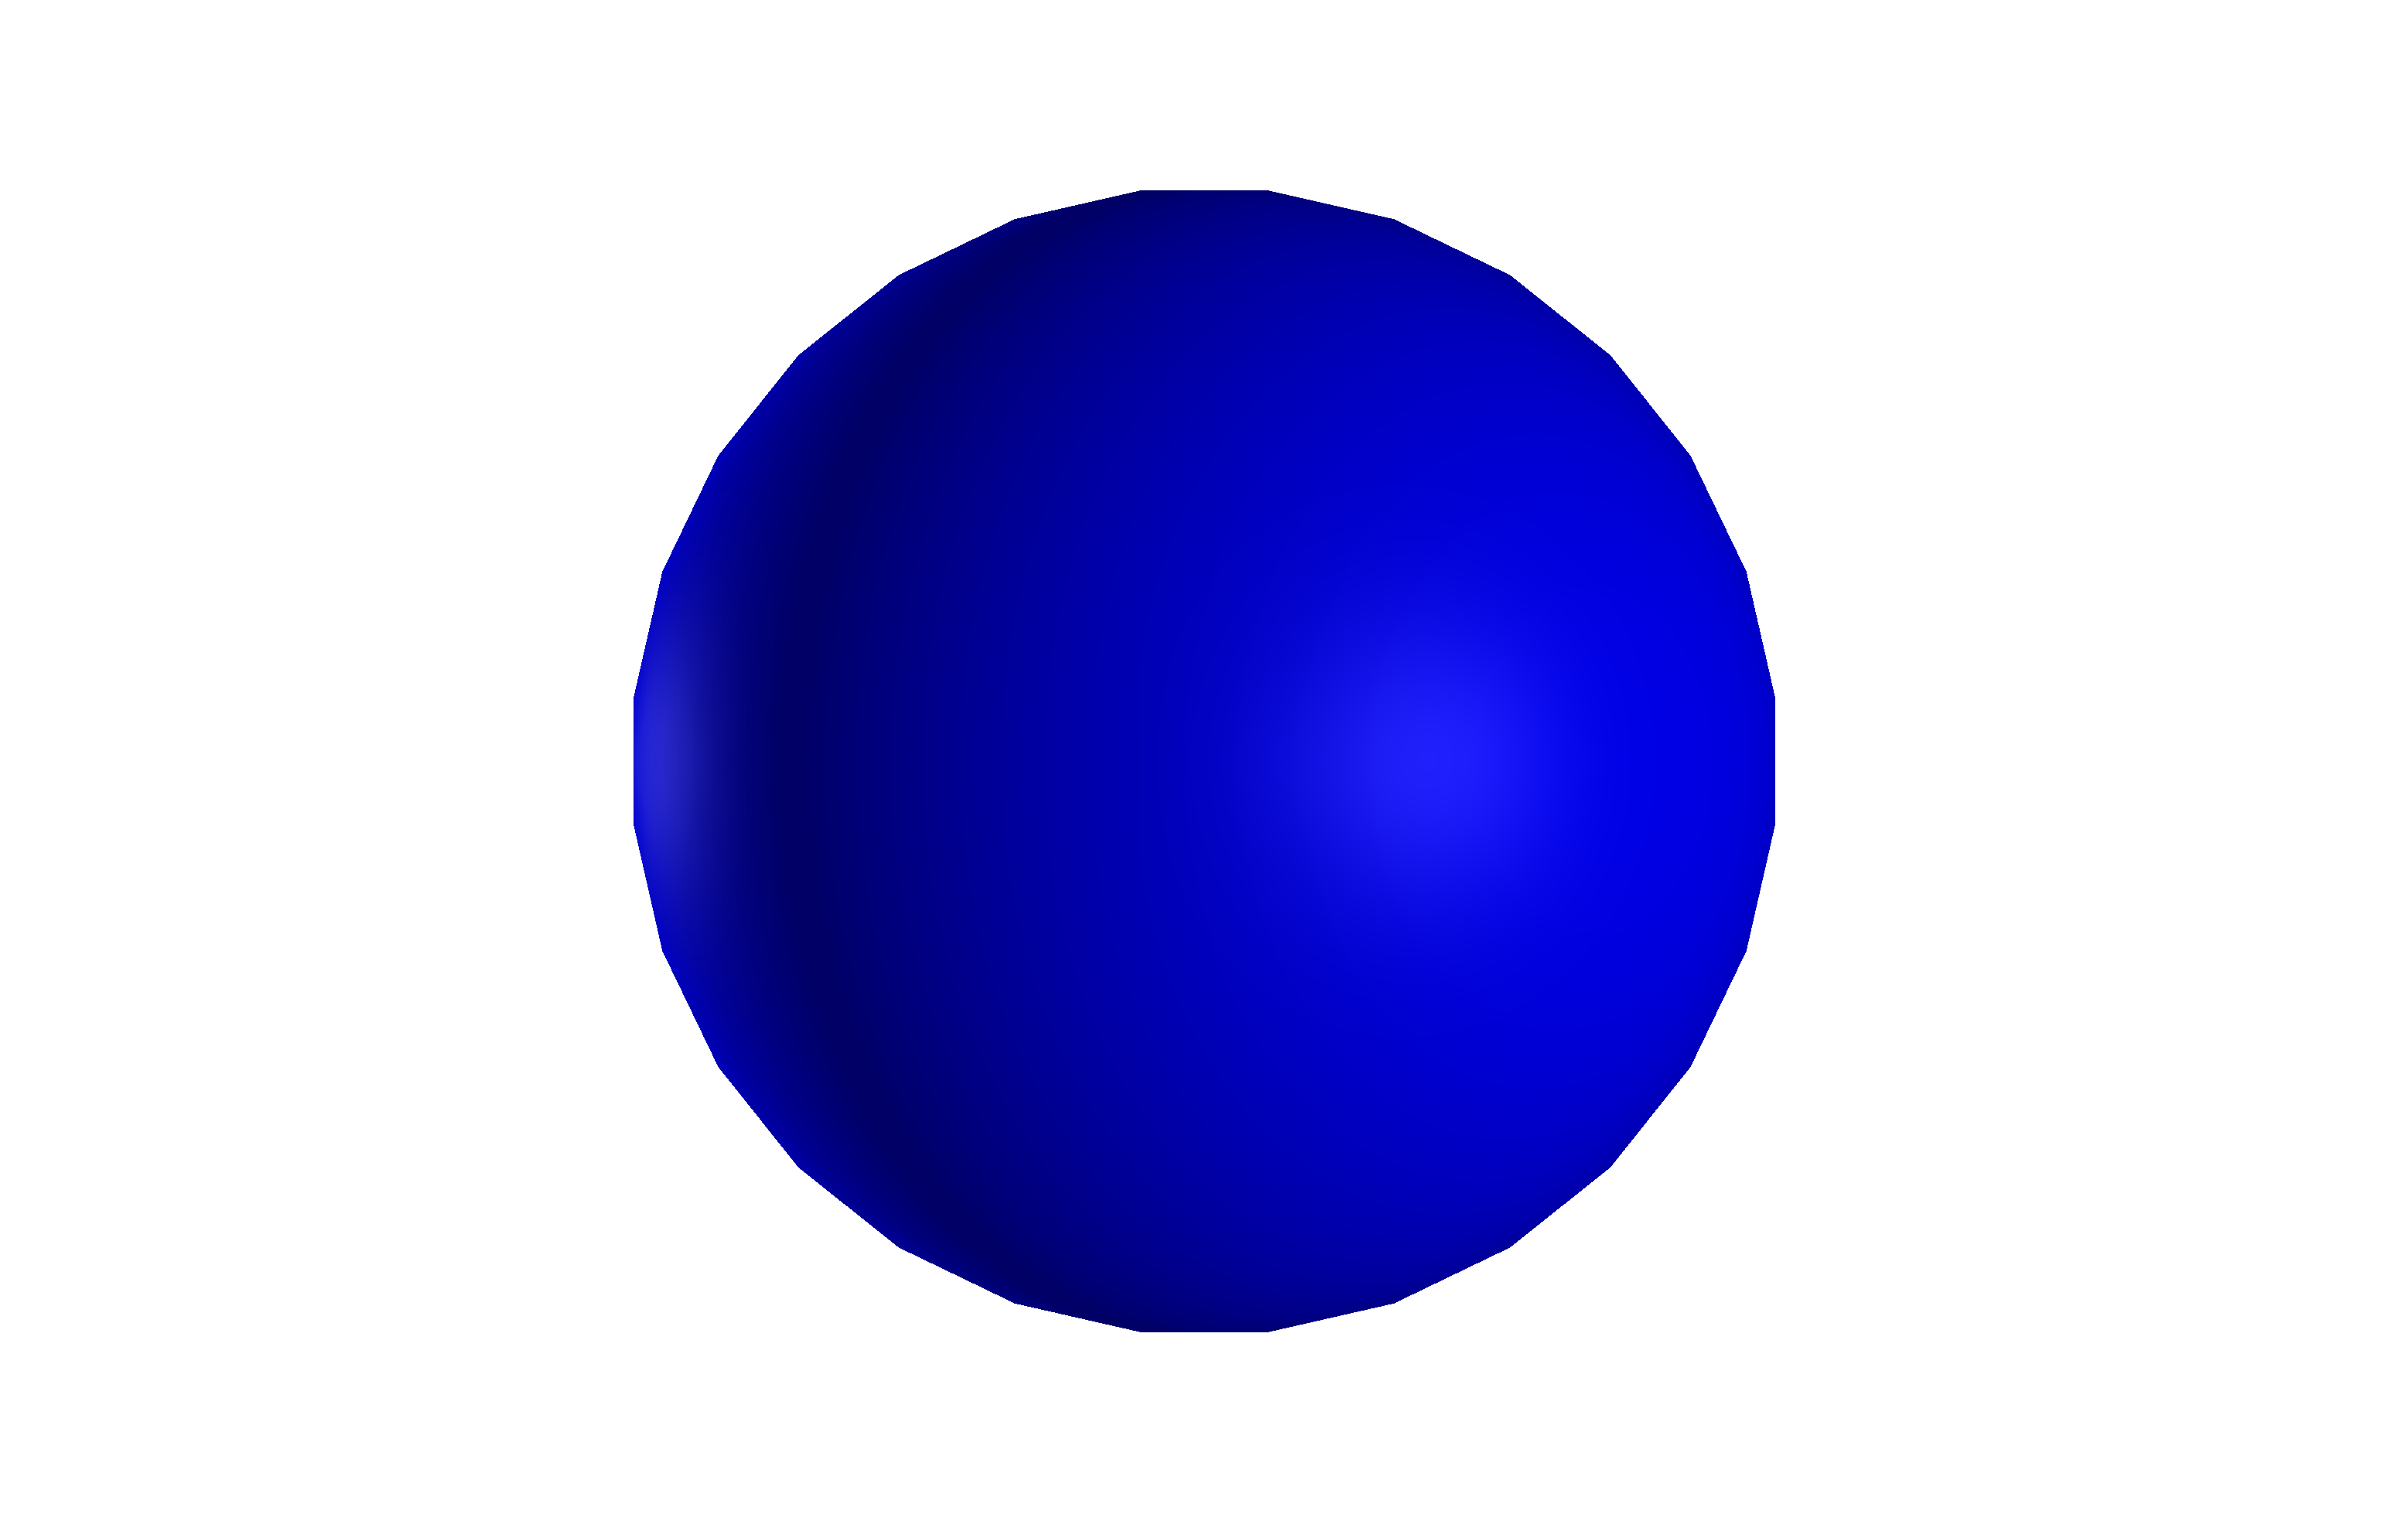
\includegraphics[width=\textwidth]{assets/images/lod/3}
      \caption{Full detail.}
      \label{fig:lod_3}
    \end{subfigure}
    
    \begin{subfigure}{0.3\textwidth}
      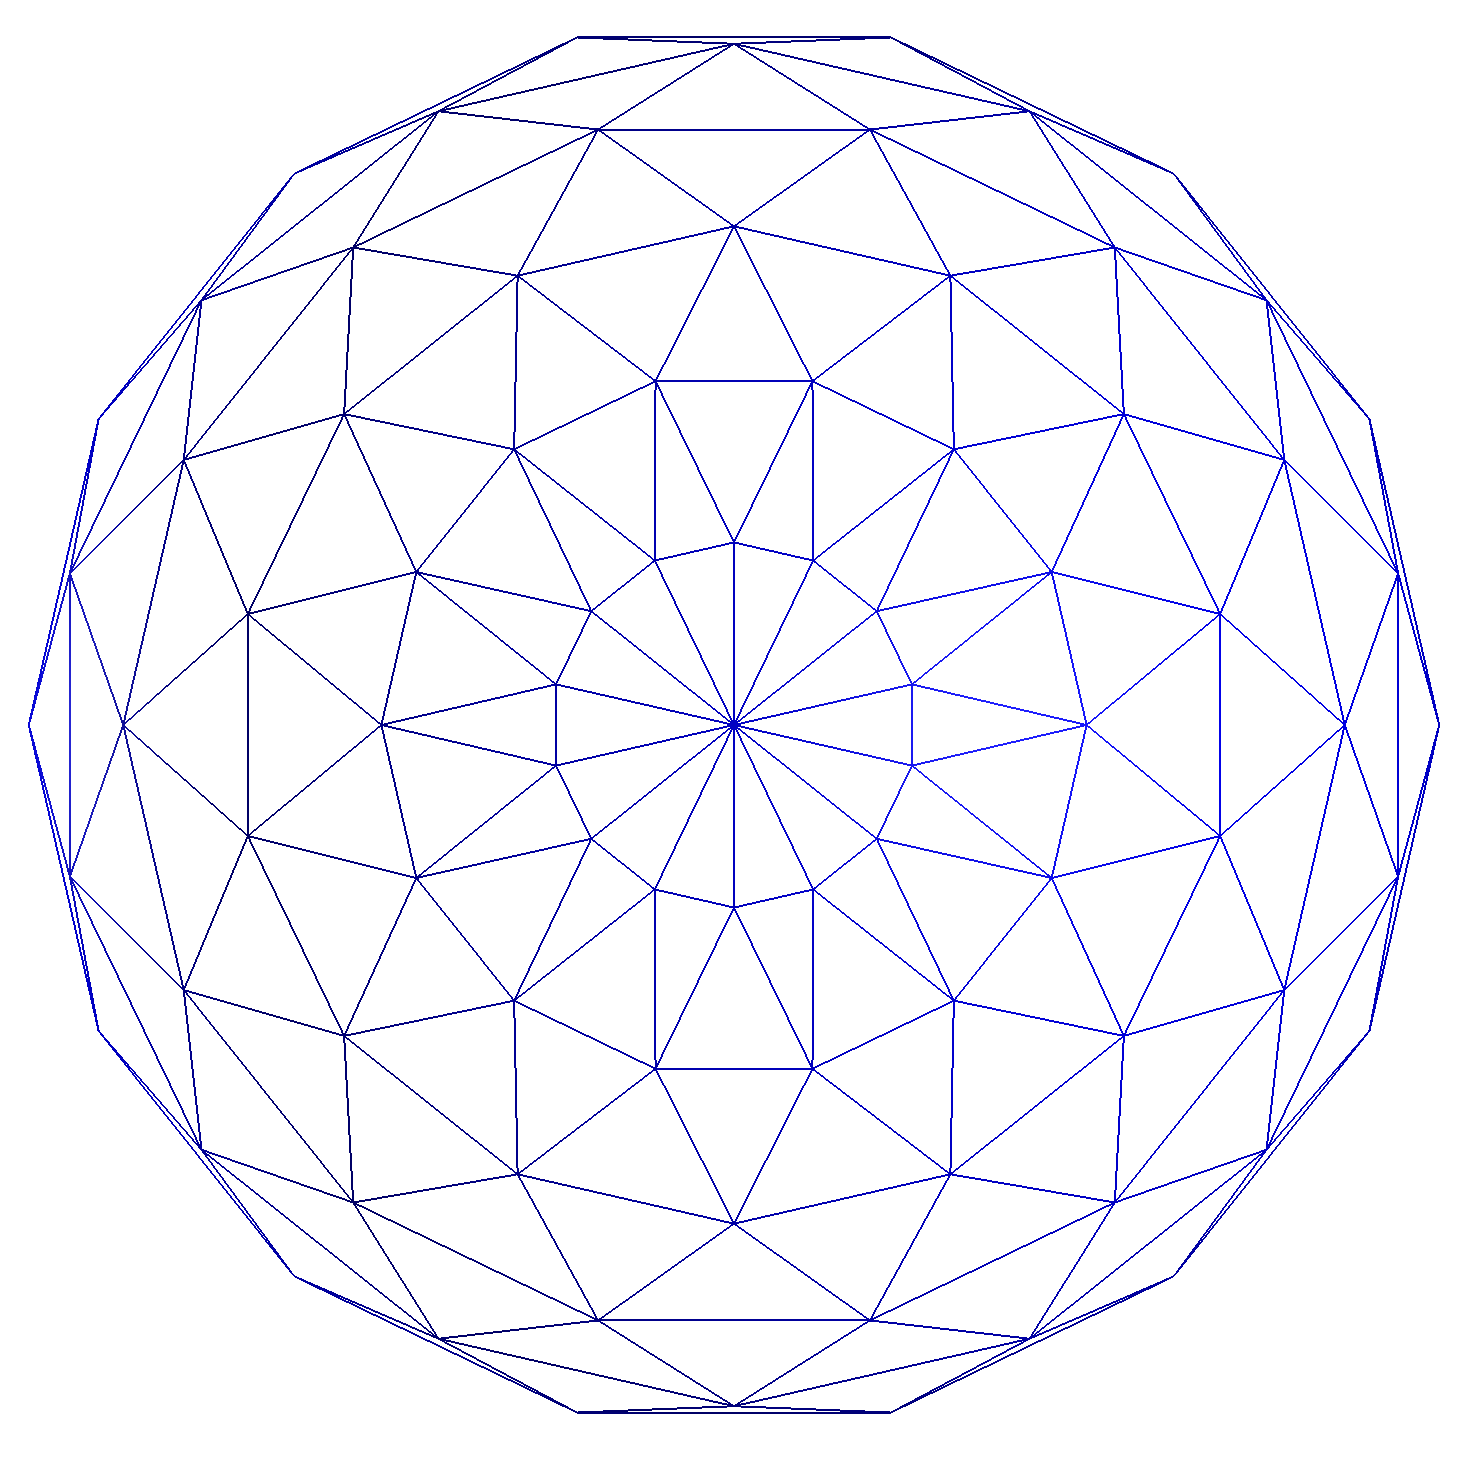
\includegraphics[width=\textwidth]{assets/images/lod/1_w}
      \caption{Low detail.}
      \label{fig:lod_1_w}
    \end{subfigure}
    \begin{subfigure}{0.3\textwidth}
      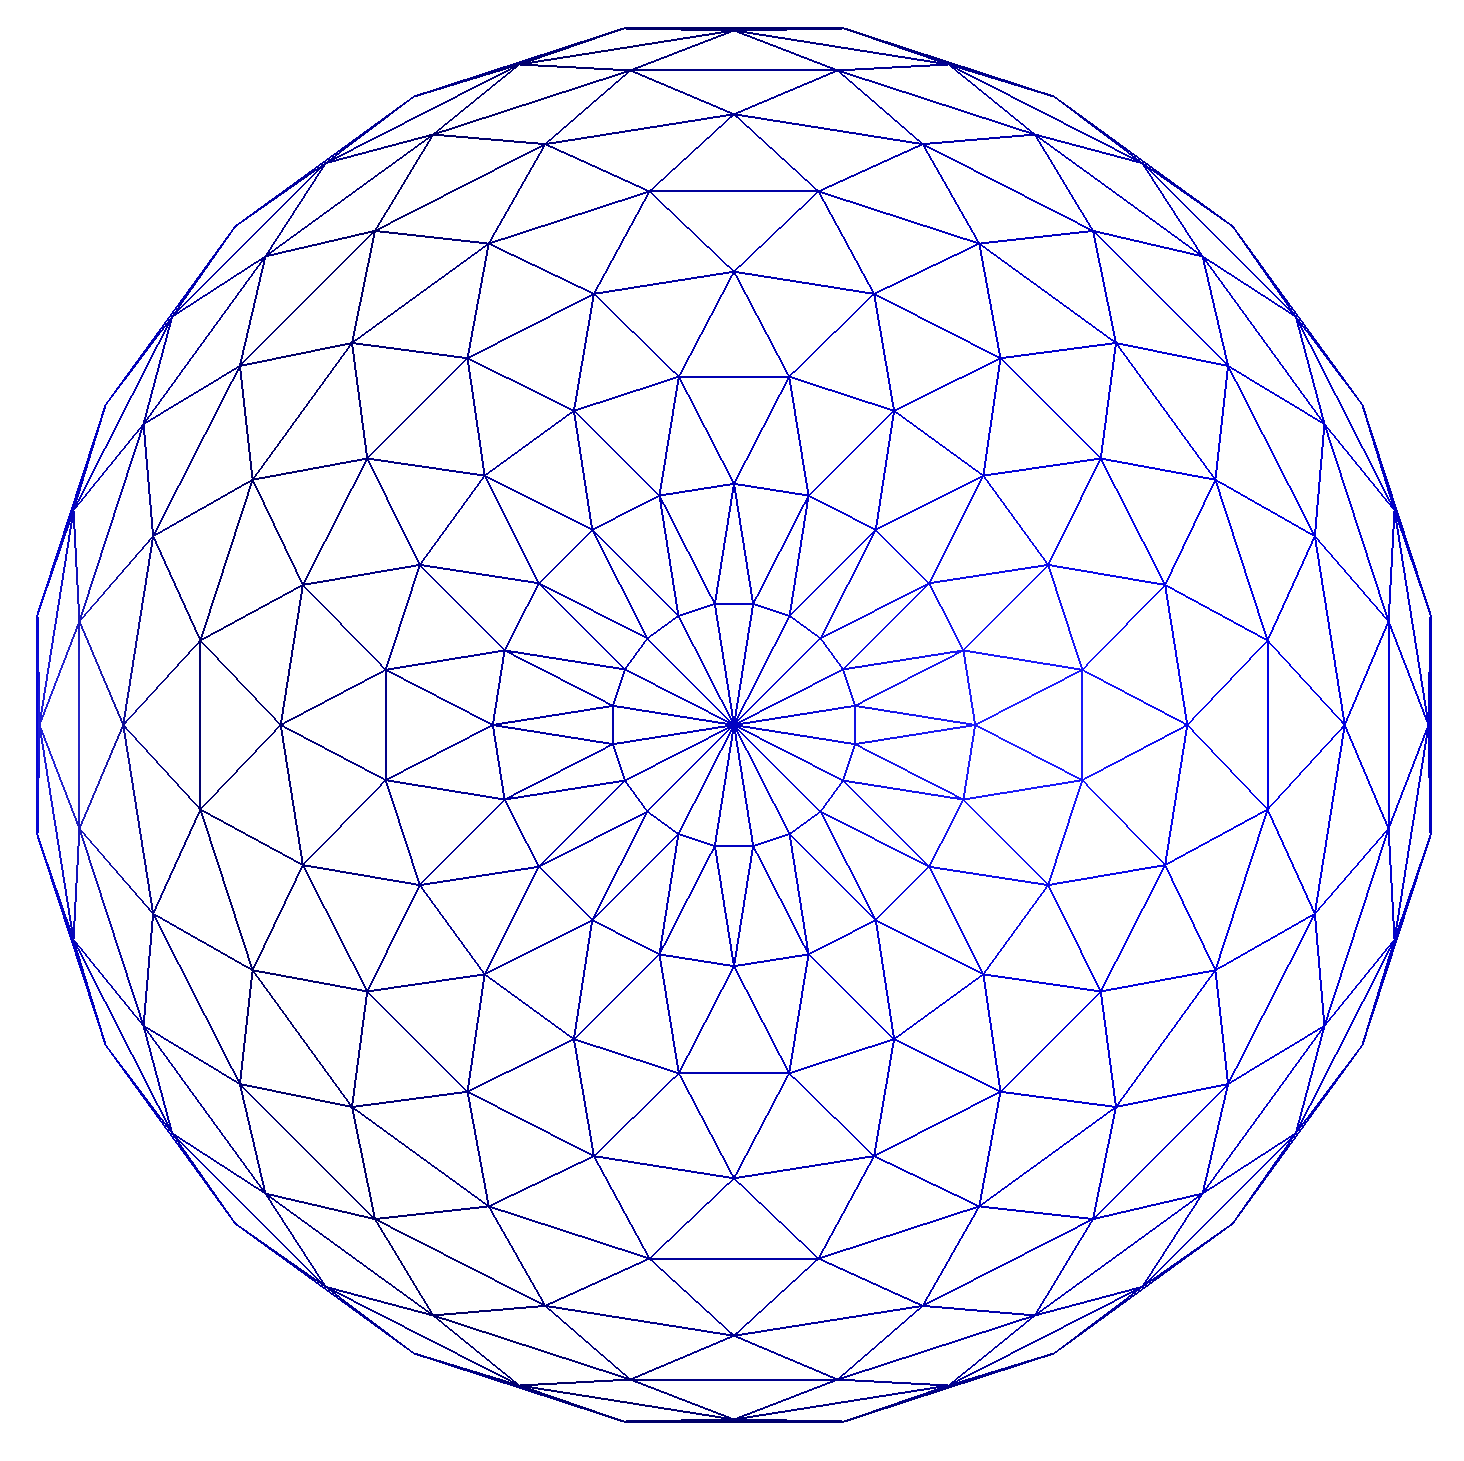
\includegraphics[width=\textwidth]{assets/images/lod/2_w}
      \caption{Medium detail.}
      \label{fig:lod_2_w}
    \end{subfigure}
    \begin{subfigure}{0.3\textwidth}
      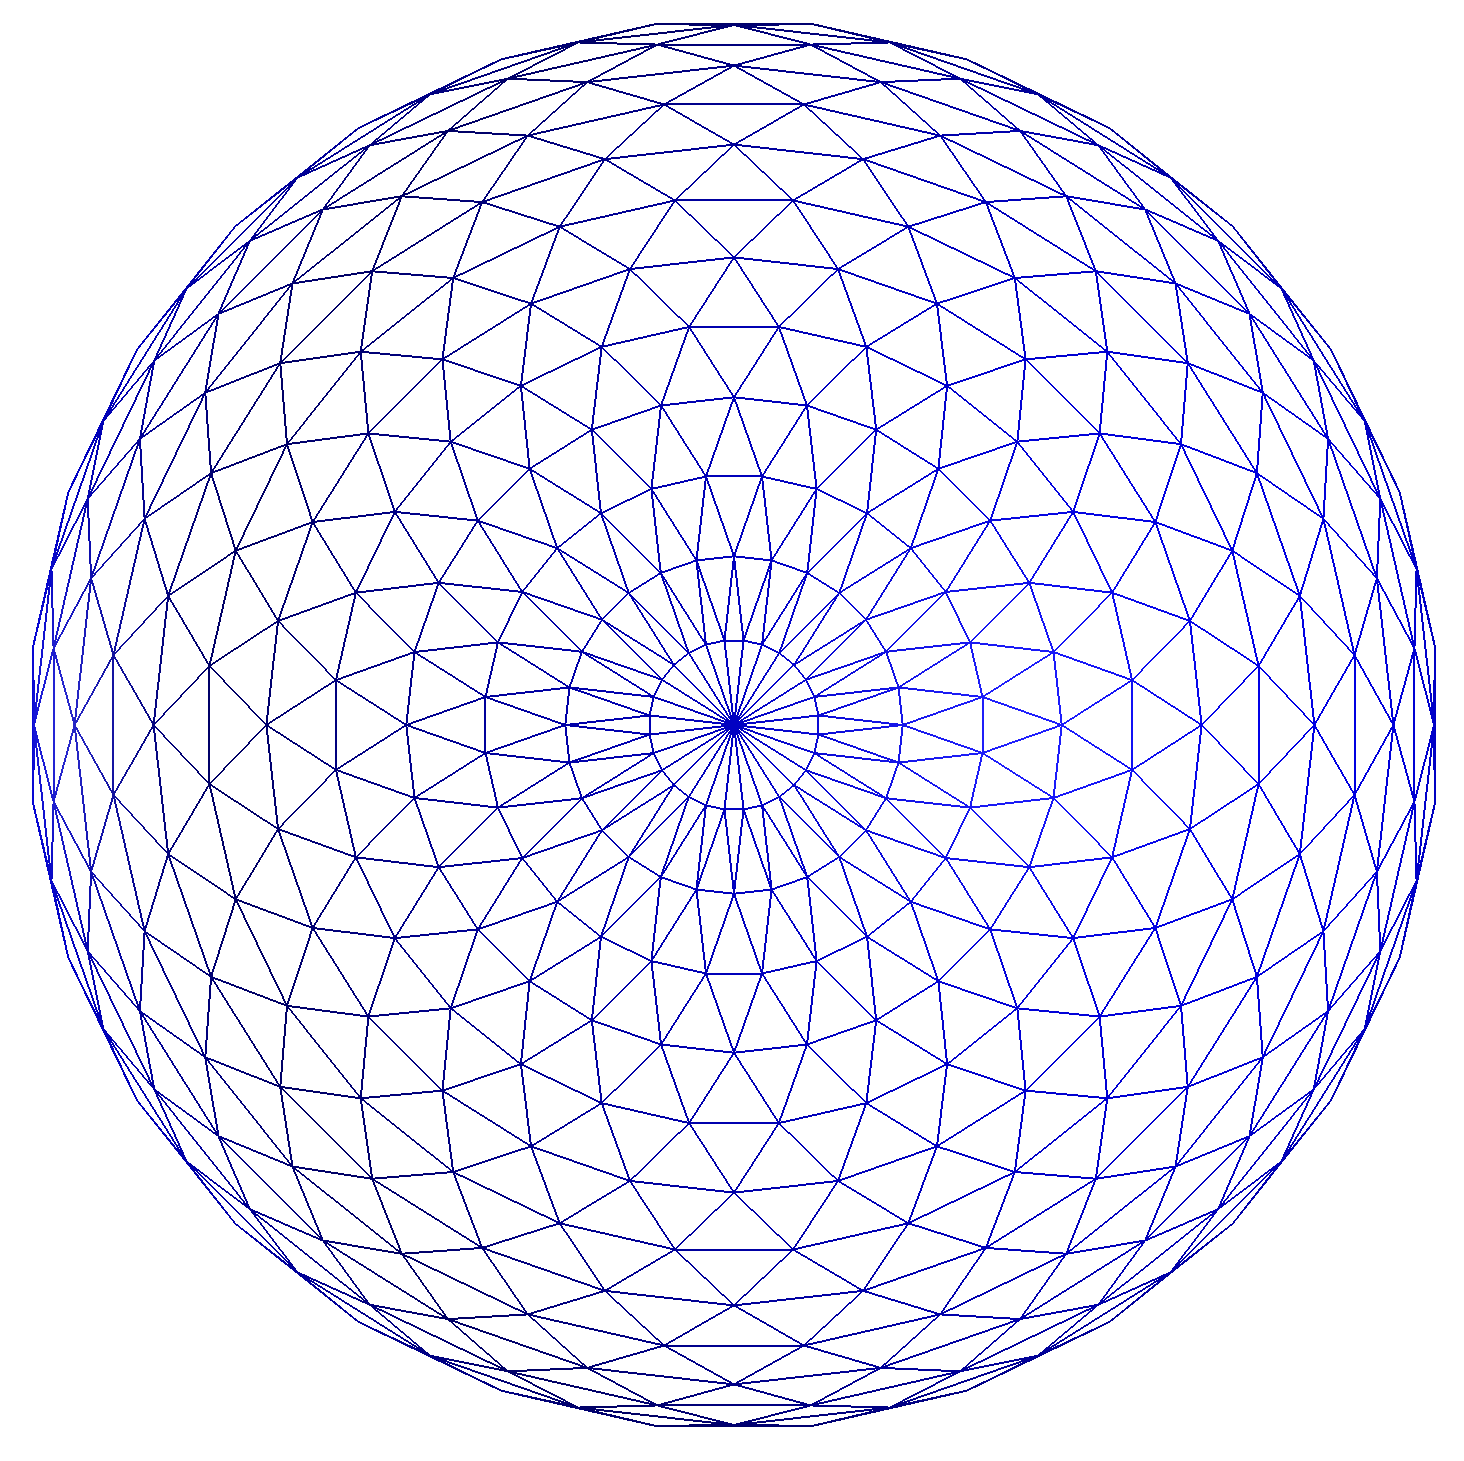
\includegraphics[width=\textwidth]{assets/images/lod/3_w}
      \caption{Full detail.}
      \label{fig:lod_3_w}
    \end{subfigure}
  \end{center}
  \caption{Model complexity is decreased at subjectively chosen camera distance thresholds with minimal visible loss in quality.}
  \label{fig:lod_distances}
\end{figure}

\begin{figure}
  \begin{center}
    \begin{subfigure}{\textwidth}
      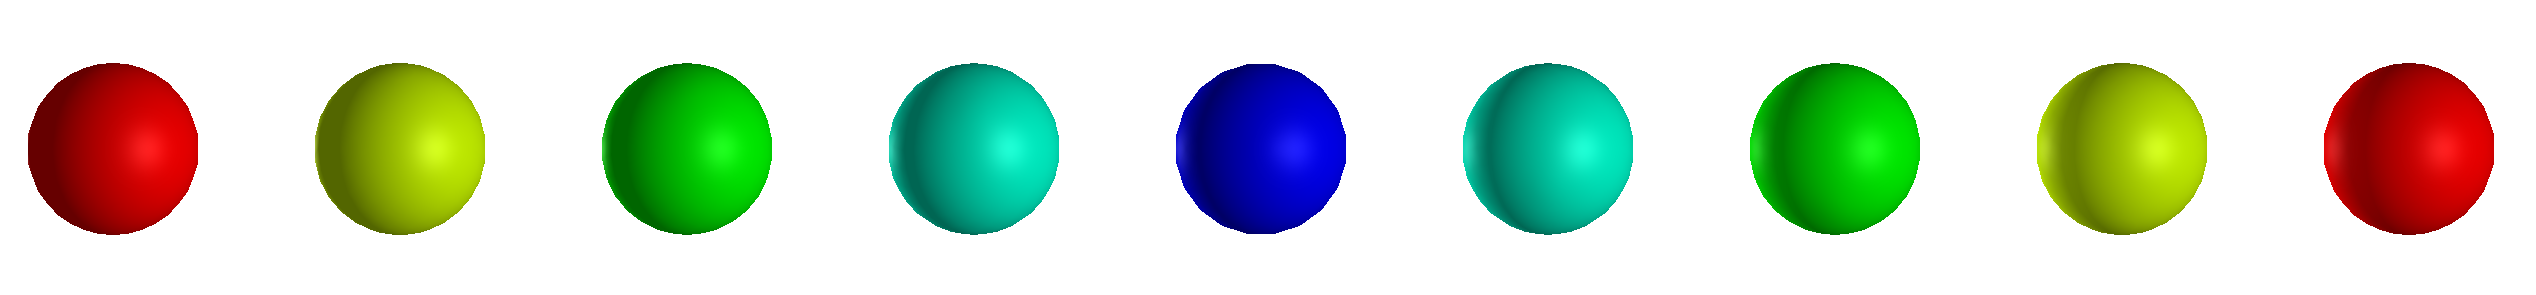
\includegraphics[width=\textwidth]{assets/images/lod/a}
      \caption{At a similar distance, all objects are identical.}
      \label{fig:lod_a}
    \end{subfigure}
    \begin{subfigure}{\textwidth}
      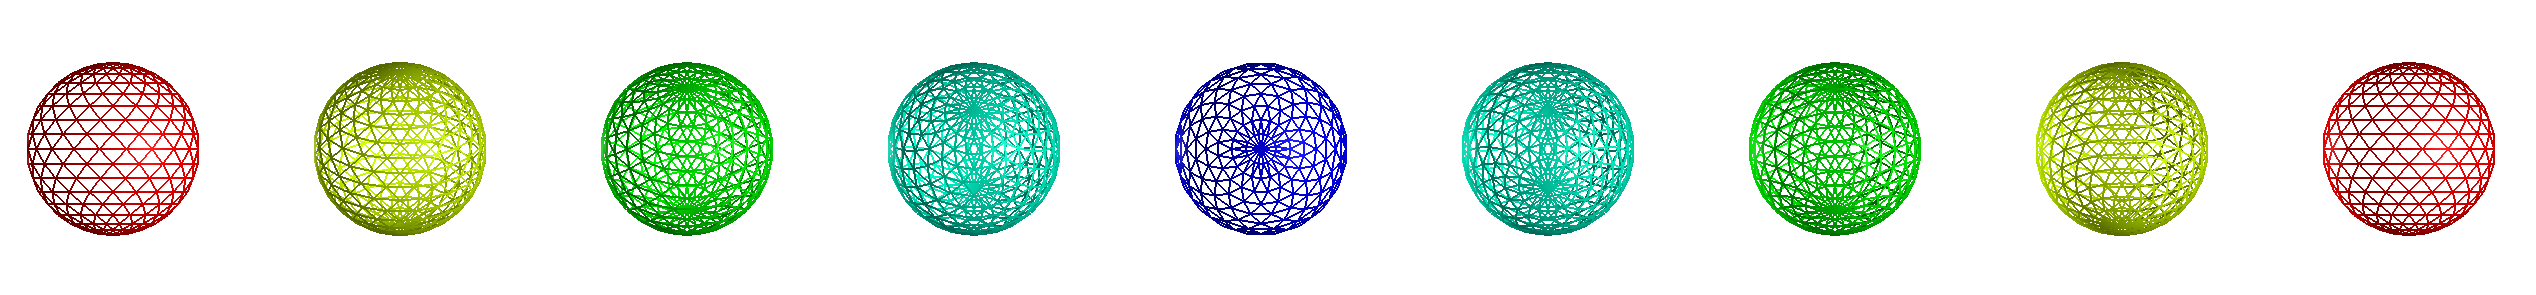
\includegraphics[width=\textwidth]{assets/images/lod/a_w}
      \caption{At a similar distance, all meshes are identical.}
      \label{fig:lod_a_w}
    \end{subfigure}
    \begin{subfigure}{\textwidth}
      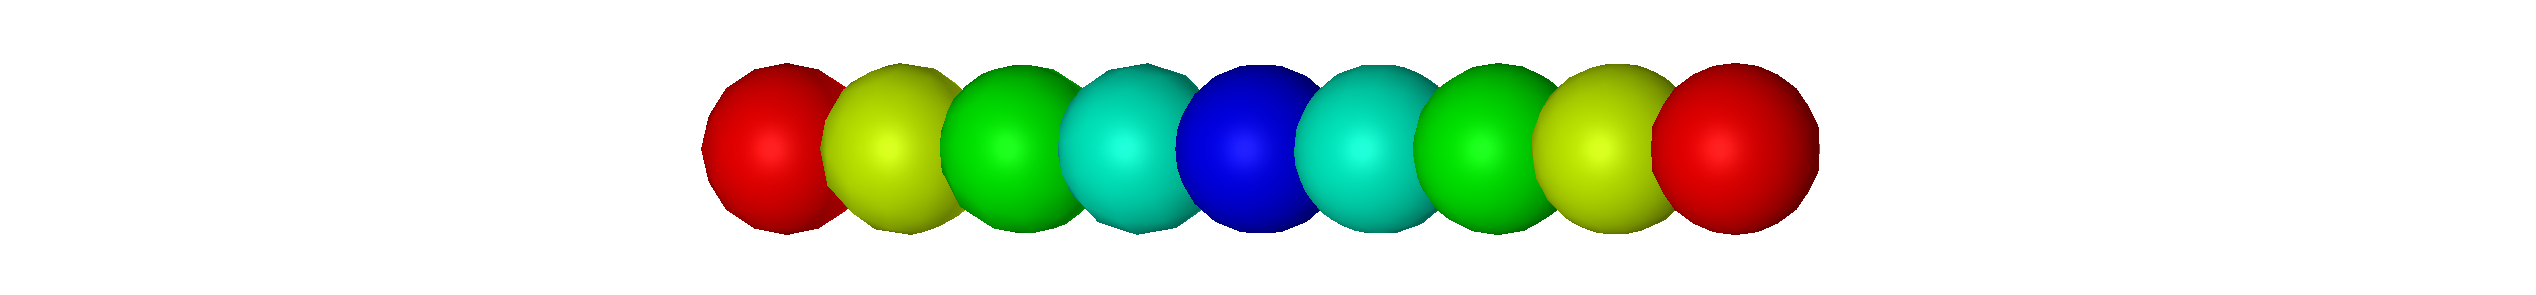
\includegraphics[width=\textwidth]{assets/images/lod/b}
      \caption{Further spheres have a minor decrease in visible quality.}
      \label{fig:lod_b}
    \end{subfigure}
    \begin{subfigure}{\textwidth}
      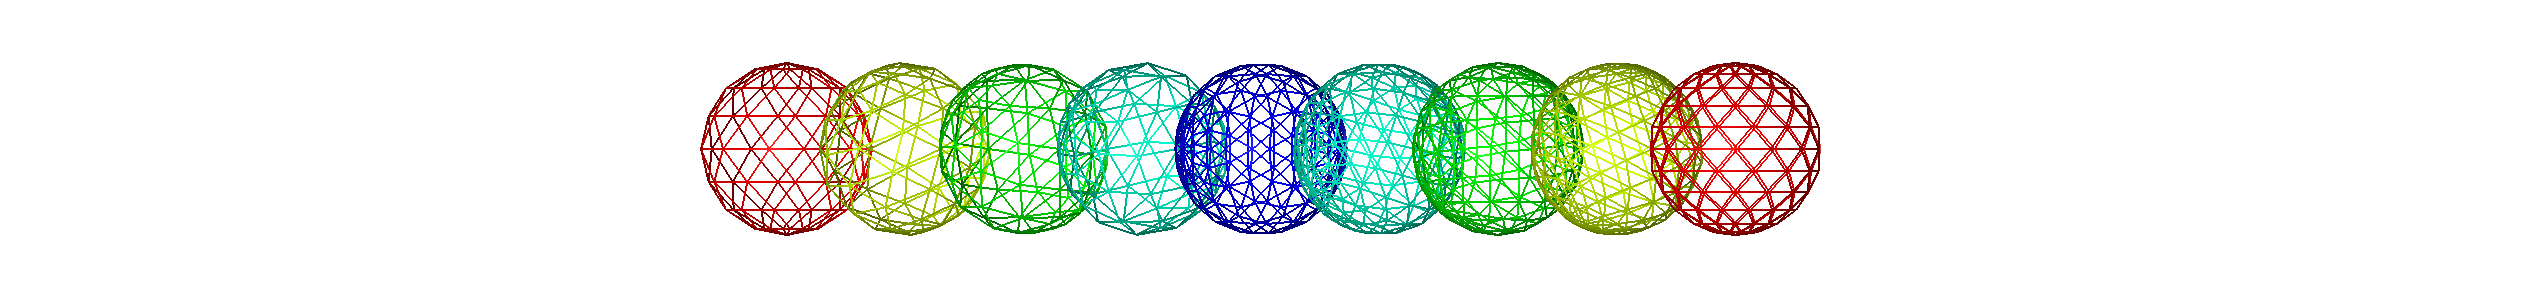
\includegraphics[width=\textwidth]{assets/images/lod/b_w}
      \caption{Further spheres have a minor decrease in triangle density.}
      \label{fig:lod_b_w}
    \end{subfigure}
  \end{center}
  \caption{Demonstration of decreased mesh quality for distant object. ``Level of Detail'' setting has been reduced below default for a more visible geometry reduction.}
  \label{fig:lod_spin}
\end{figure}

Performance analysis for this optimisation is discussed in \cref{lod_analysis_section}.
\subsection{WebMGA 3.0 Bugs}
The feature appears to work as expected, though should be tested over a wider range of scenarios to ensure LOD changes are always indistinguishable. GUI settings to change LOD distances should ideally also be implemented.
